% Created by tikzDevice version 0.12.4 on 2023-11-07 12:46:54
% !TEX encoding = UTF-8 Unicode
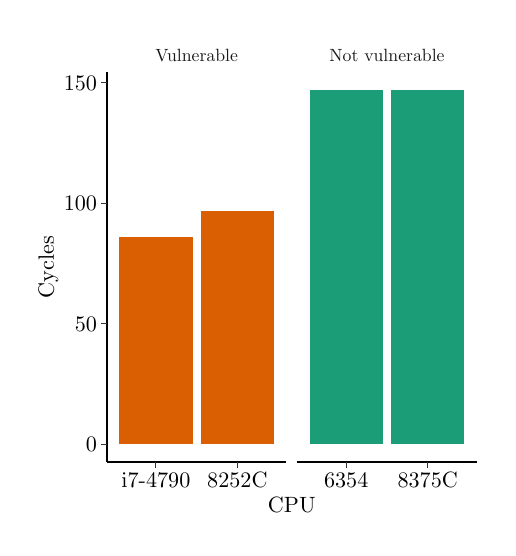
\begin{tikzpicture}[x=1pt,y=1pt]
\definecolor{fillColor}{RGB}{255,255,255}
\path[use as bounding box,fill=fillColor,fill opacity=0.00] (0,0) rectangle (166.22,180.67);
\begin{scope}
\path[clip] (  0.00,  0.00) rectangle (166.22,180.67);
\definecolor{drawColor}{RGB}{255,255,255}
\definecolor{fillColor}{RGB}{255,255,255}

\path[draw=drawColor,line width= 0.4pt,line join=round,line cap=round,fill=fillColor] (  0.00,  0.00) rectangle (166.22,180.68);
\end{scope}
\begin{scope}
\path[clip] ( 28.66, 23.73) rectangle ( 93.44,164.62);
\definecolor{fillColor}{RGB}{255,255,255}

\path[fill=fillColor] ( 28.66, 23.73) rectangle ( 93.44,164.62);
\definecolor{fillColor}{RGB}{217,95,2}

\path[fill=fillColor] ( 33.08, 30.13) rectangle ( 59.58,105.18);

\path[fill=fillColor] ( 62.52, 30.13) rectangle ( 89.02,114.55);
\end{scope}
\begin{scope}
\path[clip] ( 97.44, 23.73) rectangle (162.22,164.62);
\definecolor{fillColor}{RGB}{255,255,255}

\path[fill=fillColor] ( 97.44, 23.73) rectangle (162.22,164.62);
\definecolor{fillColor}{RGB}{27,158,119}

\path[fill=fillColor] (101.86, 30.13) rectangle (128.36,157.99);

\path[fill=fillColor] (131.30, 30.13) rectangle (157.80,158.22);
\end{scope}
\begin{scope}
\path[clip] ( 28.66,164.62) rectangle ( 93.44,176.68);
\definecolor{drawColor}{gray}{0.10}

\node[text=drawColor,anchor=base,inner sep=0pt, outer sep=0pt, scale=  0.64] at ( 61.05,168.45) {Vulnerable};
\end{scope}
\begin{scope}
\path[clip] ( 97.44,164.62) rectangle (162.22,176.68);
\definecolor{drawColor}{gray}{0.10}

\node[text=drawColor,anchor=base,inner sep=0pt, outer sep=0pt, scale=  0.64] at (129.83,168.45) {Not vulnerable};
\end{scope}
\begin{scope}
\path[clip] (  0.00,  0.00) rectangle (166.22,180.67);
\definecolor{drawColor}{RGB}{0,0,0}

\path[draw=drawColor,line width= 0.6pt,line join=round] ( 28.66, 23.73) --
	( 93.44, 23.73);
\end{scope}
\begin{scope}
\path[clip] (  0.00,  0.00) rectangle (166.22,180.67);
\definecolor{drawColor}{gray}{0.20}

\path[draw=drawColor,line width= 0.4pt,line join=round] ( 46.33, 21.73) --
	( 46.33, 23.73);

\path[draw=drawColor,line width= 0.4pt,line join=round] ( 75.77, 21.73) --
	( 75.77, 23.73);
\end{scope}
\begin{scope}
\path[clip] (  0.00,  0.00) rectangle (166.22,180.67);
\definecolor{drawColor}{RGB}{0,0,0}

\node[text=drawColor,anchor=base,inner sep=0pt, outer sep=0pt, scale=  0.80] at ( 46.33, 14.62) {i7-4790};

\node[text=drawColor,anchor=base,inner sep=0pt, outer sep=0pt, scale=  0.80] at ( 75.77, 14.62) {8252C};
\end{scope}
\begin{scope}
\path[clip] (  0.00,  0.00) rectangle (166.22,180.67);
\definecolor{drawColor}{RGB}{0,0,0}

\path[draw=drawColor,line width= 0.6pt,line join=round] ( 97.44, 23.73) --
	(162.22, 23.73);
\end{scope}
\begin{scope}
\path[clip] (  0.00,  0.00) rectangle (166.22,180.67);
\definecolor{drawColor}{gray}{0.20}

\path[draw=drawColor,line width= 0.4pt,line join=round] (115.11, 21.73) --
	(115.11, 23.73);

\path[draw=drawColor,line width= 0.4pt,line join=round] (144.55, 21.73) --
	(144.55, 23.73);
\end{scope}
\begin{scope}
\path[clip] (  0.00,  0.00) rectangle (166.22,180.67);
\definecolor{drawColor}{RGB}{0,0,0}

\node[text=drawColor,anchor=base,inner sep=0pt, outer sep=0pt, scale=  0.80] at (115.11, 14.62) {6354};

\node[text=drawColor,anchor=base,inner sep=0pt, outer sep=0pt, scale=  0.80] at (144.55, 14.62) {8375C};
\end{scope}
\begin{scope}
\path[clip] (  0.00,  0.00) rectangle (166.22,180.67);
\definecolor{drawColor}{RGB}{0,0,0}

\path[draw=drawColor,line width= 0.6pt,line join=round] ( 28.66, 23.73) --
	( 28.66,164.62);
\end{scope}
\begin{scope}
\path[clip] (  0.00,  0.00) rectangle (166.22,180.67);
\definecolor{drawColor}{RGB}{0,0,0}

\node[text=drawColor,anchor=base east,inner sep=0pt, outer sep=0pt, scale=  0.80] at ( 25.06, 27.38) {0};

\node[text=drawColor,anchor=base east,inner sep=0pt, outer sep=0pt, scale=  0.80] at ( 25.06, 70.94) {50};

\node[text=drawColor,anchor=base east,inner sep=0pt, outer sep=0pt, scale=  0.80] at ( 25.06,114.50) {100};

\node[text=drawColor,anchor=base east,inner sep=0pt, outer sep=0pt, scale=  0.80] at ( 25.06,158.07) {150};
\end{scope}
\begin{scope}
\path[clip] (  0.00,  0.00) rectangle (166.22,180.67);
\definecolor{drawColor}{gray}{0.20}

\path[draw=drawColor,line width= 0.4pt,line join=round] ( 26.66, 30.13) --
	( 28.66, 30.13);

\path[draw=drawColor,line width= 0.4pt,line join=round] ( 26.66, 73.70) --
	( 28.66, 73.70);

\path[draw=drawColor,line width= 0.4pt,line join=round] ( 26.66,117.26) --
	( 28.66,117.26);

\path[draw=drawColor,line width= 0.4pt,line join=round] ( 26.66,160.82) --
	( 28.66,160.82);
\end{scope}
\begin{scope}
\path[clip] (  0.00,  0.00) rectangle (166.22,180.67);
\definecolor{drawColor}{RGB}{0,0,0}

\node[text=drawColor,anchor=base,inner sep=0pt, outer sep=0pt, scale=  0.80] at ( 95.44,  5.56) {CPU};
\end{scope}
\begin{scope}
\path[clip] (  0.00,  0.00) rectangle (166.22,180.67);
\definecolor{drawColor}{RGB}{0,0,0}

\node[text=drawColor,rotate= 90.00,anchor=base,inner sep=0pt, outer sep=0pt, scale=  0.80] at (  9.51, 94.18) {Cycles};
\end{scope}
\end{tikzpicture}
